\documentclass[pdftex,12pt,letter]{article}
\usepackage[binary-units=true]{siunitx}
\usepackage[margin=0.75in]{geometry}
\usepackage{verbatim}
\usepackage{graphicx}
\usepackage{cite}
\usepackage{color}
\usepackage[pdftex,pdfpagelabels,bookmarks,hyperindex,hyperfigures]{hyperref}
\usepackage{xspace}
\usepackage{amssymb}


\bibliographystyle{unsrt}

\newcommand{\fixme}[1]{\textbf{FIXME: #1}}    
\newcommand{\pd}{protoDUNE\xspace}

\title{A Proposal for the Single-Phase \pd Experiment Data Challenges in 2017-2018}
\date{\today}
\author{R.Pordes, M.Potekhin, R.Sulej}

\begin{document}


\maketitle

\begin{abstract}



\noindent It is important to ensure 100\% readiness of the
end-to-end \pd software and computing complex during the detector commissioning period and
throughout data taking in 2018. We propose to conduct two Data Challenges (DCs) in order to identify
and address potential issues before they can impact the experiment. 
\par
The Data Challenges will be done with the
understanding that the software is not in the final state for beam running. 
\par
DCs will include defining and  testing interfaces, measuring rates and reliability of data transfers and job execution, understanding the set of processing workflows, and publishing the results of monitoring the infrastructure as well as the physics outputs.


Version 1: May 2017 - Initial definition of components of the data challenges
\par

Version 2: In progress. Will be used to initially define and agree on the components of DC1. Add some consistent numbering/naming of the steps to be done. Add information on files used/needed.

\end{abstract}

\tableofcontents

\pagebreak

\section{About this document}
%There are two main factors that make it necessary to ensure 100\% readiness of the
%end-to-end \pd software and computing complex during the detector commissioning period and
%throughout data taking in 2018. First, due to the short run schedule spending any significant amout
%of time on debugging will make fulfillment of
%the run plan impossible. Second, the Collaboration will need to process and analyze the NP04 data
%on a reasonably short time scale (months rather than years) in order to maximize benefits of the
%prototype effort for the DUNE R\&D work and CDR cycle, so efficient resource management and
%throughput of \pd processing will be of essence right at the beginning of data taking. For these
%reasons, and given the \pd schedule,  we propose to conduct two Data Challenges in order to identify
%and address potential issues before they can impact the experiment.

The goal of this document is to provide concise information about the proposed \pd Data Challenges
to the individual working groups in order to coordinate effort and come to a consensus as to the scope,
plans and schedule of the proposed Data Challenges. \textit{It does not contain detailed descriptions
and/or designs of the \pd computing
infrastructure elements} and the reader is reffered to existing documentation where
needed, with references provided in the text.

\section{The Scope of the Data Challenges}
Information regarding the \pd (NP04) computing is summarized in the \pd-SP Technical Design Report\cite{docdb1794}.

\subsection{Components}
The following components (including infrastructure, middleware and software) can be identified as relevant in the context
of Data Challenges (which will be also referred to as \textit{``DC''} in this document):
\begin{enumerate}
\item The DAQ \textbf{Online Buffer} which stores raw data assembled by the Event Builders, as files on disk. The internals
of the DAQ system itself are not within the scope.

\item  \textbf{Beam Instrumentation Interface}. Most of the Beam Instrumentation data is not included into the data stream
handled by the \pd DAQ (whose primary task is to capture data from the TPC and the Photon Detector), and is instead
transmitted to the Beam Instrumentation Database at CERN. It is not available immediately for each triggered event,
and is instead available in batches after each spill cycle of the SPS. Interfacing this system is a task that needs
to be addressed for \pd to be able to include these data in its offline processing in an optimal manner.
%validate its beam trigger system.

% Adding Online Monitoring based on talking to Christos/Flavio and as a test for writing to the git repository
% Ruth, July 31st 2017
\item The \textbf{Slow Control and Online Monitoring System} which provide control, monitoring and display of the data acquisition readout and detector parameters. 

\item The \textbf{Data Management System}\cite{docdb1212}  which performs data transfers between a few endpoints
at CERN and FNAL starting with the Online Buffer, including output from DQM,  and which is also tasked with proper accounting and handling of the file catalog and other metadata
by interacting with the SAM system at FNAL (see next item). The Data Management/Handling System will also interface the disk-based mass storage
at CERN and FNAL (i.e.\,EOS\cite{eos} and dCache) as well as tape systems (CASTOR and Enstore respectively).
We anticipate using the \textit{Fermi File Transfer System} (also abbreviated as F-FTS\cite{fts}).

\item The \textbf{File Catalog (Metadata)}  -- SAM system at FNAL which comprises the functionality of the file catalog, data storage and
retrieval based on Metadata and can also be used for orchestration of production workflows.

\item \textbf{Data Quality Monitoring} (DQM) which is tasked with running algorithms with turnaround time short enough to provide
actionable results (under and hour) but which won't fit into the computational footprint of the Online Monitoring (a part of DAQ).
To support DQM, the ProtoDUNE Prompt Processing System (\textbf{p3s}) \cite{docdb1811,p3s} has been created and will run any type of\
DQM workload as formulated and programmed by the working groups.

\item \textbf{Calibration} While it is not expected that these components will be finalized
(and some even exist) at the time of the first Data Challenge it is important to have a firm grasp of the required interfaces,
data flow patterns and other crucial aspects of the \pd Calibration software.
 \item \textbf{Reconstruction}. While it is not expected that these components will be finalized
(and some even exist) at the time of the first Data Challenge it is important to have a firm grasp of the required interfaces,
data flow patterns and other crucial aspects of the \pd Reconstruction Systems. Having prototypes in place is therefore crucial
on the time scale of the Data Challenges.
An important component of the overall production chain is the \textit{Data Reduction} step along the lines described
in \cite{docdb2089}. It combines a few signal-processing procedures (cf. digital filtering and noise reduction), and it will be
necessary in any version or architecture of the production software.
Understanding the interfaces and practical implications of this component would be a useful part of the Data Challenge.

\item \textbf{Analysis Suite Prototypes}. Same comment applies here as to the previous item, i.e.\,while there is no expectation
for the final design and implementation of the analysis chain to exist early in the experiment (especially that it is by nature the most
dynamic and fluid part of all software) it is important to put in place, document and optimize its interfaces with various components
of infrastructure e.g.\,calibration databases, Metadata, software and data provenance controls etc.

\item \textbf{Production Operations Management System (based on POMS)}. This FNAL-based service includes using the DUNE service portal, production workflows executed by POMS \cite{poms}, including the management and automation of  jobs
submission on distributed resources on the Grid. It will be the primary platform for \pd on which to run production and analysis.


\end{enumerate}
\noindent The relationship between the various infrastructure and other components listed above is schematically illustrated in
Fig.\ref{fig:dc1}. This diagram relflects the fact that transmission of \pd data is a multistage process and in particular there
will be separate instances of F-FTS transferring the data from the Online Buffer to mass storage at CERN, and then from
CERN to FNAL and elsewhere.

\begin{figure}[tbh]
  \centering
  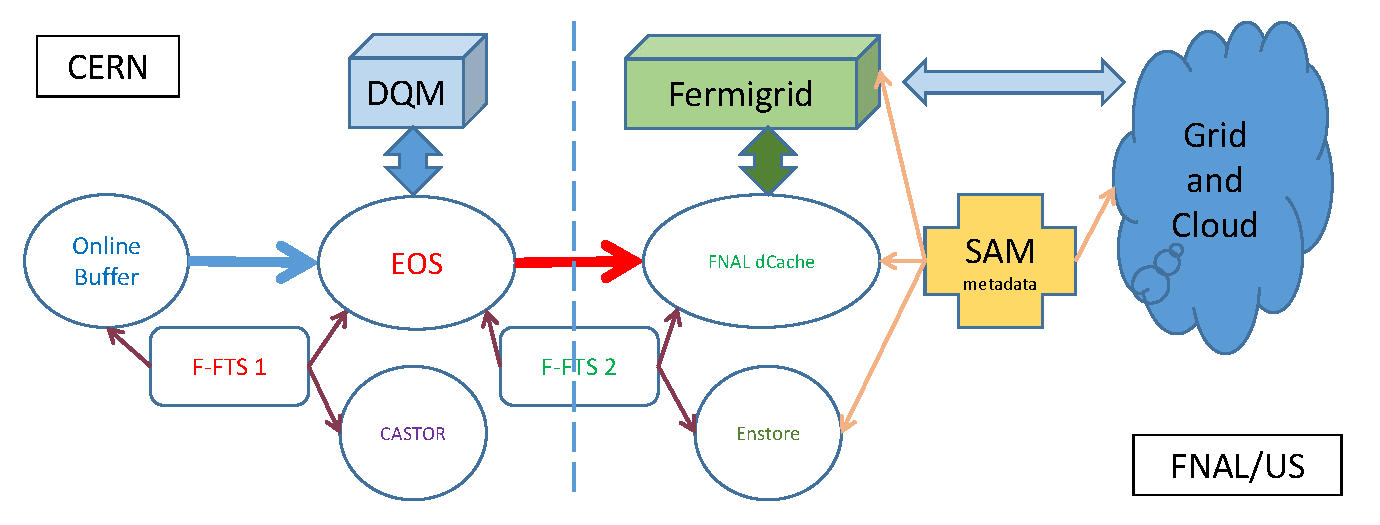
\includegraphics[width=1.0\textwidth]{../figures/data_challenge_1.pdf}
  \caption{Schematics of data flow and  processing in \pd data challenges.}
  \label{fig:dc1}
\end{figure}
\noindent Data and production streams which belong to \pd Monte Carlo simulation domain are not included in the
scope of Data Challenges presented here.



\subsection{Files and Interfaces: ** Incomplete/Wrong  - For Discussion **}


The information here will be built up as needed and known. In general it will be pointers to existing documentation  internal to the appropriate components. 
\renewcommand{\theenumi}{\alph{enumi}}
\begin{enumerate}
\item Beam Instrumentation Database Interface - data format and name of code module and description of the database attributes and internface.
\item Calibration data  -  data format and name of code module and description of the database attributes and interface for calibration information.
\item DQM output files - information about files output from DQM, their location, type and internal format.
\item Input data file - any directory and file naming conventions and details as well as scripts that use this information
\item Input data format - internal format of an input data file
\item POMS configuration files - means of access to and editing of POMS requests.
\item Reduced data format - location of reduced data files (if any) and description of their internal format
\item SAM metadata files  - what SAM metadata files are needed and their description.
\item Slow Control data format - data format and name of code module and description of the database attributes and interface for slow control information.
\end{enumerate}
\renewcommand{\theenumi}{\alph{arabic}}

An ongoing diagram of the workflows and their dependencies is shown in Figure 2: Schematic of Dependencies. It is another aim of the data challenges to check that terminology, and it's presentation, is consistent across components - work to be done!

\begin{figure}[tbh]
  \centering
  \includegraphics[width=1.0\textwidth]{integration.png}
  \caption{Schematic of Dependencies}
  \label{fig:dependencies}
\end{figure}



\subsection{Work-up to the Data Challenges}
Before any end-to-end data challenge can be meaningful, all individual components and interfaces must undergo
their own functional testing. The scope of the pre-DC activity will include most of the components above and an understanding of what files, file and data formats, and interfaces are going to be used. An initial list is given below and will be modified as things are better understood.
\begin{itemize}

\item \textbf{Slow Control and Online Monitoring}

\item \textbf{Data Transfer and SAM interaction}.  Both F-FTS1 and F-FTS2 components as schematically depicted in Fig.\,\ref{fig:dc1}
must undergo end-to-end functional testing including registration in SAM and sinking data to tape storage both at CERN and FNAL. A test
agent will be created which simulates creation of the raw data files by DAQ, which are written to the Online Buffer and picked up
by the F-FTS for transmission.

\item \textbf{Beam Instrumentation Interface}. At a minimum, prototype schemas for \pd beam detectors must be created in
the CERN Beam Instrumentation Database, and populated with dummy data. An extraction process must be put in place which
``captures'' these data and commits it either to a database managed by \pd and/or as files on disk (EOS). A prototype
of the merging process must be put in place. This will also require data access libraries to be utilized in the production process.

\item  \textbf{DQM/p3s}. The prompt processing system must be tested and validated to run with the primary data
staging area being in EOS. The issues of deployment, updating and maintenance of LArSoft and other requisite software
must be resolved.

\item  \textbf{Data Reduction Software}.
% In one shape or another, data reduction will form a distinct stage in the production chain  in \pd.
A prototype of this software module must be tested with simulated data and packaged in a way that is portable across
FNAL and facilities at CERN.

\item  \textbf{Calibration}
Prototypes of this software need to be put in place. They will
include components specific to LArTPC, the Photon Detector and the Beam Instrumentation data, which will also require
merging and processing.
\item \textbf{Production Software} Prototypes of this software need to be put in place. They will
include components specific to LArTPC, the Photon Detector and the Beam Instrumentation data, which will also require
merging and processing.

\item  \textbf{Production Management and Support}. This includes running prototypes of this software utilizing the FNAL POMS.

\item  \textbf{Analysis}. The main point in this exercise to to ready the interface of the analysis software to SAM and other
components of the production system(s). There are no strict requirements to functionality and performance of the analysis
software at this stage.

\end{itemize}
\noindent  One of the goals of the work-up period is to identify components that overlap and where software can be shared and reused. 

\subsection{Collaboration Tools, Reporting and Documentation}
We are using a mail list (DUNE-proto-sp-dc), DUNE SLACK channel (pd-sp-datachallenges) for planning and technical details.  Documentation to be retained will be submitted to the DUNE DocDB. Results/summary of the data challenge for the will be posted to the DUNE wiki.

\clearpage

\section{Data Challenge 1}

Data Challenge 1 (DC1) is taking place the week of November 6th. It is currently not sure when/how the Cold Box Test schedule for initial data taking overlaps with this week.  It is important for the Data Challenge not to perturb the needs for the Cold Box Test. 

\begin{itemize}

\item Provide Input Data: 
\begin{itemize}
\item Simulated raw data files will be deposited into a Test/Simulated Online Buffer by a specially created test agent.
\item  Initially this will be on a CERN OpenStack VM for testing of functionality but not performance. 
\item A script will be written to deposit or cycle through several files. 
\end{itemize}
\item SAM Metadata is created for the files either by hand or through a script

\item The data files are automatically detected by F-FTS-Lite and transmitted to EOS.

\item The input data files are transferred to storage at Fermilab and CERN and declared to the file catalog.
\begin{itemize}
\item F-FTS initiates data transfer to dCache and Enstore at FNAL. 
\item F-FTS initiated data transfer to Castor
\item Files are updated in SAM
\end{itemize}

\item Beam Instrumentation data is captured by \pd systems and is stored either on a DB server or as files on EOS.
These data do not need to be real at this point, as the purpose of this step is to test interfaces and protocols.


\item Automated process initiates DQM streams in p3s. In DC1, full-blown processing on CERN Tier-0\,\cite{lxbatch}
will not be required and at a minimum the operation of p3s will be validated on the Neutrino Platform cluster\,\cite{neut}.

\item Production team at FNAL submits production jobs using the newly arrived data as input. This includes prototype interfaces
to software components of the LArTPC, Photon Detector and Beam Instrumentation systems.

\end{itemize}

DC1 s  defined and will be done independently from the Cold Box Test, while clearly  benefiting from the work being done for it. If the DAQ group leaders agree at the time,  stretch goals of the Data Challenge will be to move: statically placed simulated data files from the online buffer through the system; and, if detector data does become available in time, statically placed acquired data files statically placed in the online disk buffer.

\clearpage

\section{Data Challenge 2}
This will be listed nearer the date - at the moment sometime in March 2018.
%\begin{itemize}
%\item DAQ sends raw data (such as pulser or simulated trigger data) to the Online Bufer.
%\item The data is detected by F-FTS1 and transmitted to EOS.
%\item F-FTS2 initiates data transfer to dCache at FNAL. Contact is made with the Metadata system (SAM) where the files are registered.
%\item Realistic Beam Instrumentation data is captured by \pd systems and is stored either on a DB server or as files on EOS.
%\item Automated process initiates DQM streams in p3s using  CERN Tier-0. At a minimum, ADC and noise spectra (FFT) are produced and delivered to the user by a Web service.
%\item Production team at FNAL submits production jobs using the newly arrived data as input. Interfaces between software components,
data etc as well as actual functionaltiy are close to final.
%\item Analysis chain is activated.
%\end{itemize}


%\section{Personnel and Responsibilities}
%\color{red} This list is currently being revised. \color{black}
%\begin{itemize}
%\item Online Buffer and the test agent -- DAQ team
%\item Beam Instrumentation Interface -- Beam Instrumentation Group, DB coordinator: J.Paley
%\item F-FTS -- FNAL team (lead: A.Norman)
%\item p3s -- prompt processing team (lead: M.Potekhin)
%\item DQM and production payloads -- DRA team (co-leads: D.Stefan, R.Sulej)
%\item Calibrations -- M.Mooney
%\item Integration consultant -- B.Viren
%\item Metadata and SAM -- FNAL SCD (T.Junk, S.Fuess)
%\item Production support at CERN and FNAL -- TBD
%\item Analysis -- TBD
%\item Coordination -- R.Pordes
%\end{itemize}

\clearpage


\begin{thebibliography}{1}

\bibitem{docdb1794}
{DUNE DocDB 1794: \textit{ProtoDUNE-SP Technical Design Report }}\\
\url{http://docs.dunescience.org:8080/cgi-bin/ShowDocument?docid=1794}



\bibitem{docdb1212}
{DUNE DocDB 1212: \textit{Design of the Data Management System for the protoDUNE Experiment}}\\
\url{http://docs.dunescience.org:8080/cgi-bin/ShowDocument?docid=1212}

\bibitem{eos}
{The CERN Exabyte Scale Storage}\\
\url{http://information-technology.web.cern.ch/services/eos-service}


\bibitem{fts}
{The Fermilab File Transfer System}\\
\url{http://cd-docdb.fnal.gov/cgi-bin/RetrieveFile?docid=5412&filename=datamanagement-changeprocedures.pdf&version=1}


\bibitem{docdb1811}
{DUNE DocDB 1811: \textit{Prompt Processing System Requirements for the Single-Phase protoDUNE}}\\
\url{http://docs.dunescience.org:8080/cgi-bin/ShowDocument?docid=1811}

\bibitem{p3s}
{A Design of the Prompt Processing System for the Single-Phase protoDUNE experiment (NP04 )}\\
\url{http://docs.dunescience.org:8080/cgi-bin/ShowDocument?docid=1861}

\bibitem{docdb2089}
{Proposed Initial Data Reduction for protoDUNE/SP}\\
\url{http://docs.dunescience.org/cgi-bin/RetrieveFile?docid=2089}

\bibitem{poms}
{Production Operations Management Service (POMS)}\\
\url{https://cdcvs.fnal.gov/redmine/projects/prod_mgmt_db}


\bibitem{lxbatch}
{The CERN batch computing service}\\
\url{http://information-technology.web.cern.ch/services/batch}



\bibitem{neut}
{Neutrino Computing Cluster at CERN}\\
\url{https://twiki.cern.ch/twiki/bin/view/CENF/NeutrinoClusterCERN}




\end{thebibliography}


\end{document}

%%% Local Variables:
%%% mode: latex
%%% TeX-master: t
%%% End:
\grid
